\documentclass[12pt]{article}
\usepackage{times} 			% use Times New Roman font

\usepackage[margin=1in]{geometry}   % sets 1 inch margins on all sides
\usepackage{hyperref}               % for URL formatting
\usepackage[pdftex]{graphicx}       % So includegraphics will work
\setlength{\parskip}{1em}           % skip 1em between paragraphs
\usepackage{indentfirst}            % indent the first line of each paragraph
\usepackage{datetime}
\usepackage[small, bf]{caption}
\usepackage{listings}               % for code listings
\usepackage{xcolor}                 % for styling code
\usepackage{multirow}

%New colors defined below
\definecolor{backcolour}{RGB}{246, 246, 246}   % 0xF6, 0xF6, 0xF6
\definecolor{codegreen}{RGB}{16, 124, 2}       % 0x10, 0x7C, 0x02
\definecolor{codepurple}{RGB}{170, 0, 217}     % 0xAA, 0x00, 0xD9
\definecolor{codered}{RGB}{154, 0, 18}         % 0x9A, 0x00, 0x12

%Code listing style named "gcolabstyle" - matches Google Colab
\lstdefinestyle{gcolabstyle}{
  basicstyle=\ttfamily\small,
  backgroundcolor=\color{backcolour},   
  commentstyle=\itshape\color{codegreen},
  keywordstyle=\color{codepurple},
  stringstyle=\color{codered},
  numberstyle=\ttfamily\footnotesize\color{darkgray}, 
  breakatwhitespace=false,         
  breaklines=true,                 
  captionpos=b,                    
  keepspaces=true,                 
  numbers=left,                    
  numbersep=5pt,                  
  showspaces=false,                
  showstringspaces=false,
  showtabs=false,                  
  tabsize=2
}

\lstset{style=gcolabstyle}      %set gcolabstyle code listing

% to make long URIs break nicely
\makeatletter
\g@addto@macro{\UrlBreaks}{\UrlOrds}
\makeatother

% for fancy page headings
\usepackage{fancyhdr}
\setlength{\headheight}{13.6pt} % to remove fancyhdr warning
\pagestyle{fancy}
\fancyhf{}
\rhead{\small \thepage}
\lhead{\small HW4, Tomar}  % EDIT THIS, REPLACE # with HW number
\chead{\small CS 532, Spring 2023} 

%-------------------------------------------------------------------------
\begin{document}

% EDIT THE ITEMS HERE
\begin{centering}
{\large\textbf{HW2 - Exploring Social Networks}}\\ 
Prashant Tomar\\
03/12/2023\\
\end{centering}

%-------------------------------------------------------------------------

% The * after \section just says to not number the sections
\section*{Q1. Friendship Paradox on Facebook.}



\subsection*{Answer}

This Task is divided into multiple steps to get the required output 

\emph{Step 1: What is the mean, standard deviation, and median of the number of friends that the user's friends have?}

The friends count were already provided by the Professor in csv File.
This code loads a dataset of friend counts from a CSV file using the pandas library, computes various statistical measures such as mean, standard deviation, and median of the friend counts, sorts the friend counts in descending order, plots the friend counts on a horizontal bar chart with the user's friend count marked in red, and displays the mean, standard deviation, and median of the friend counts. 


%Python code highlighting
\begin{lstlisting}[language=Python, caption=Extract the URIs from the .JSON file, label=lst:copy]
import pandas as pd
import matplotlib.pyplot as plt

df = pd.read_csv('HW4-friend-count.csv')

num_friends = df['FRIENDCOUNT']

mean_friends = num_friends.mean()
std_dev_friends = num_friends.std()
median_friends = num_friends.median()

sorted_friends = num_friends.sort_values(ascending=False)

plt.barh(range(len(sorted_friends)), sorted_friends)

user_friends = 250 
plt.axvline(x=user_friends, color='r')

plt.text(user_friends+10, len(sorted_friends)-20, 'U', fontsize=12)

plt.xlabel('Number of friends')
plt.ylabel('Friend number')
plt.title('Number of friends of user\'s friends')

plt.show()

print('Mean number of friends:', mean_friends)
print('Standard deviation of number of friends:', std_dev_friends)
print('Median number of friends:', median_friends)
  
\end{lstlisting}

Figure \ref{fig:1} shows the mean, median and standard deviation.

\begin{figure}[h]
    \centering
    % trim and clip are used to crop the image, trim=left bottom right top
    % width sets max width, height will be scaled appropriately
    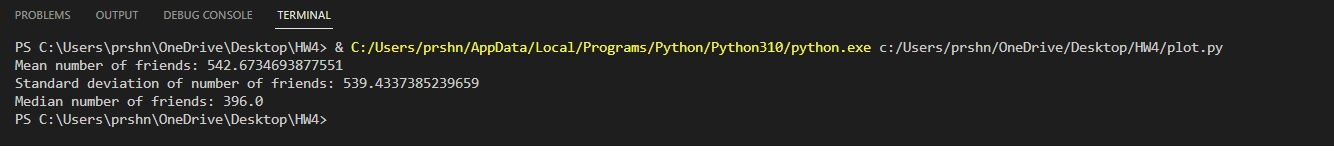
\includegraphics[trim=0 0 0 0, clip, width=1.2\textwidth,height=6cm] {2.jpg}
    \caption{Mean, Standard Deviation and Median of friends count}
    \label{fig:1}
 \end{figure}
 
Figure \ref{fig:graph} shows the graph of friends count

\begin{figure}[h]
    \centering
    % trim and clip are used to crop the image, trim=left bottom right top
    % width sets max width, height will be scaled appropriately
    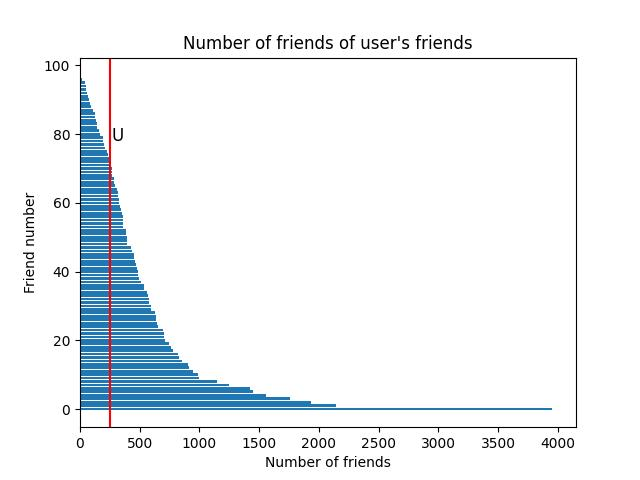
\includegraphics[trim=0 0 0 0, clip, width=1.2\textwidth,height=6cm] {1.jpeg}
    \caption{graph of friends count}
    \label{fig:graph}
\end{figure}

\emph{Step 2: Does the friendship paradox hold for this user and their friends on Facebook?}

I have observed the validity of the Friendship Paradox, which states that your friends tend to have more friends than you do. Upon examining some of my friends' Facebook profiles, I have discovered that the majority of them possess a greater number of friends than I do, although a few do no



\section*{References}
\emph Following are the references which I used while doing my HW4, you can refer to some of links from where I took help.

\begin{itemize}
    \item {DataFrame operations, \url{https://pandas.pydata.org/docs/reference/frame.html}}
    \item {Numpy, \url{https://numpy.org/doc/stable/reference/generated/numpy.log2.html/}}
    \item {Github, \url{https://github.com/odu-cs432-websci/spring23-hw4-Badjedi04}}
    \item {Python requests, \url{https://docs.python-requests.org/en/master/}}
\end{itemize}

\end{document}